\documentclass[final]{beamer}
  \mode<presentation>
  {
  \usetheme{Hitchman}
}
\usepackage{times}
\usepackage{amsmath,amssymb}
\usepackage[english]{babel}
\usepackage[latin1]{inputenc}
\usepackage[orientation=landscape,scale=2,debug]{beamerposter}  % e.g. custom size poster
  \title[Open Courses]{Open Source Courses:\\ Decision Making, Euclidean Geometry, Linear Algebra}
  \author[Hitchman]{Theron J. Hitchman}
  \institute[UNI]{University of Northern Iowa}
  \date{January 13, 2015}
  
  \pdfpageattr {/Group << /S /Transparency /I true /CS /DeviceRGB>>}
  
  \begin{document}
  \begin{frame}{} 
    \begin{columns}[t]
      \begin{column}{.31\linewidth}
       \centering
       %{\LARGE My Set-Ups}
        \begin{block}{\centering {\Large Simple Steps}}
          \centering
          {\Large
          Use Google! (Sites and Drive)\\
          Advertise with social media\\
          Share your \texttt{.tex} files\\
          }
        \end{block}
        
        \begin{block}{\centering {\Large Web Enhanced}}
         \centering
         {\Large
          \begin{itemize}
          \item HTML, CSS \& Javascript
          \item Overleaf.com\\ (Formerly writeLaTeX.com)
          \item GeoGebra
          \end{itemize}
          }
        \end{block}

        \begin{block}{\centering {\Large Advanced Open Sourcing}}
          \centering
          {\Large
          \begin{itemize}
          \item MathbookXML 
          \item Sage, SageMathCloud \\ \& Cell Server 
          \item GitHub, gh-pages, jekyll, \\ \& bootstrap
          \end{itemize}
          }
        \end{block}        
        
      \end{column}
      
       \begin{column}{.31\linewidth}
        \vspace{.15\textheight}
        \begin{block}{\centering {\Large My Core Production Tool}}
          \centering
          {\Large
          \textbf{Version Control \& File Hosting}\\ 
          git \& GitHub 
          }
        %\end{block}
        %\vspace{.05\textheight}
          %\begin{block}{\centering {\Large My Materials}}
 	 %\centering
      	 
	 \vspace{1in}
	 \centering
	 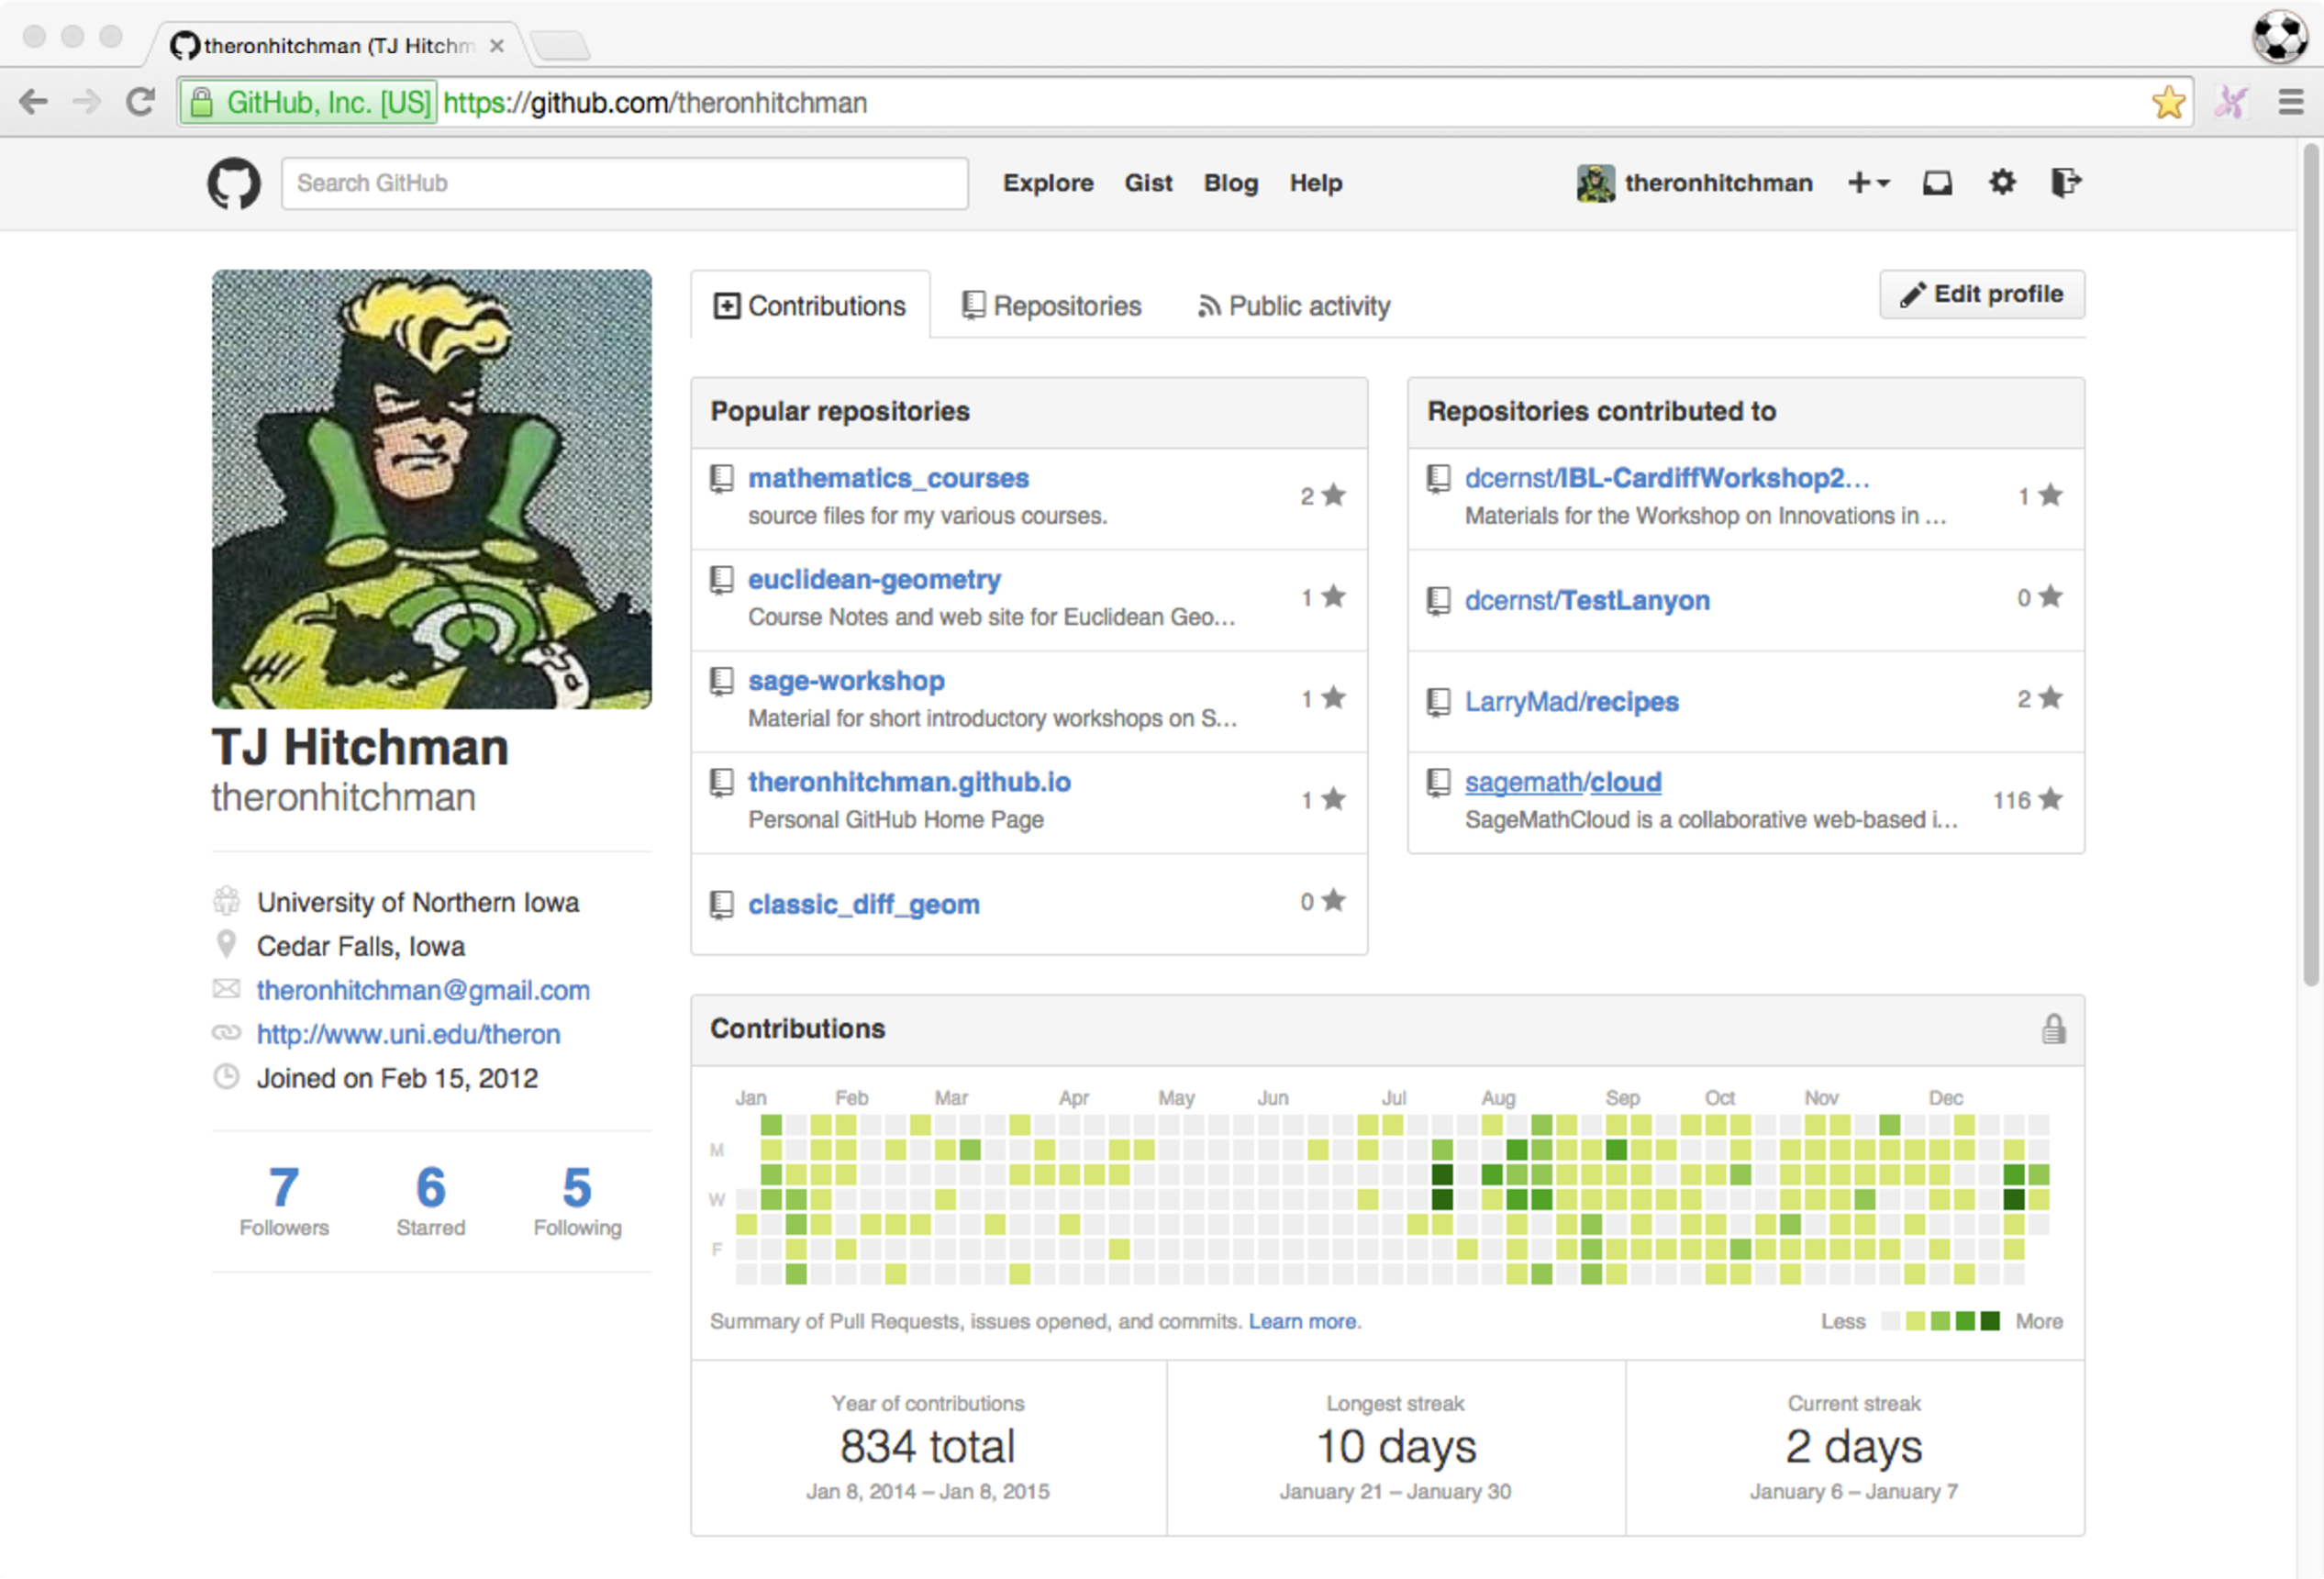
\includegraphics[width=.6\textwidth]{gh.pdf}
	 \vspace{1in} 
           \texttt{http://theronhitchman.github.io/}\\
         \end{block}
      \end{column}
      
      
      \begin{column}{.31\linewidth}
        %{\centering \LARGE My Courses}
        \begin{block}{\centering {\Large Math in Decision Making}}
            \centering
            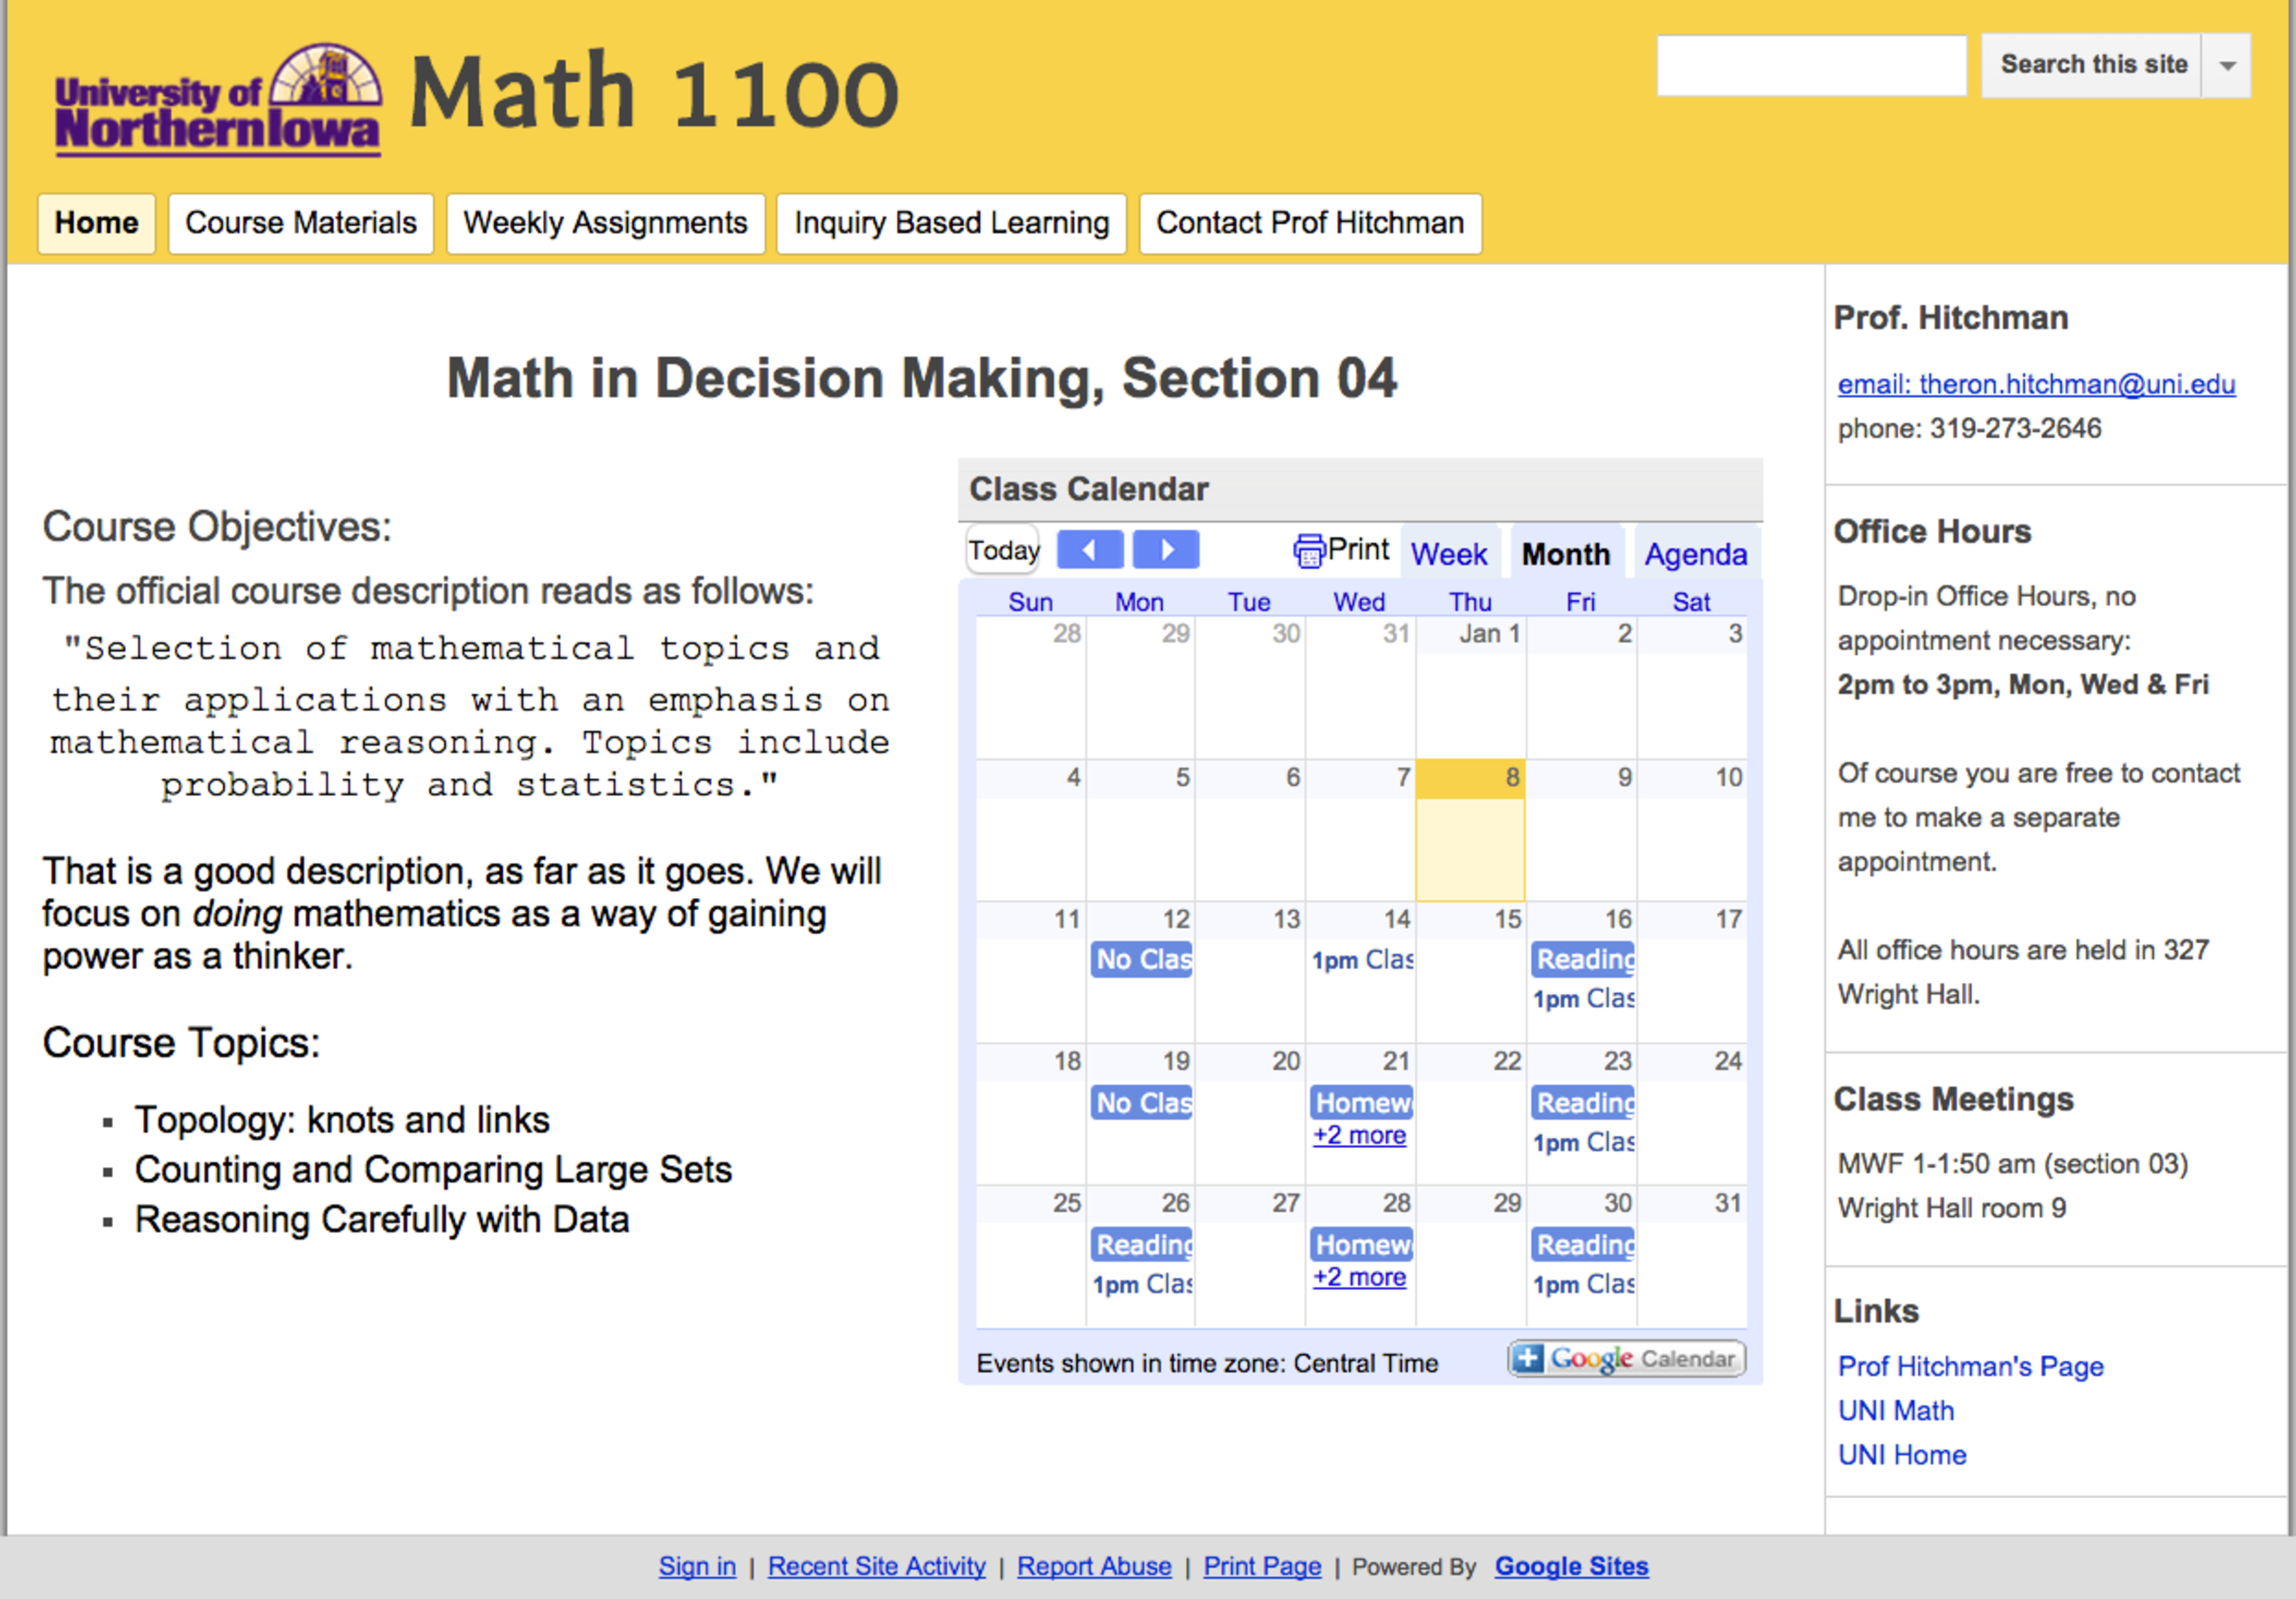
\includegraphics[width=.5\linewidth]{decisionmakingweb}
         \end{block}

        \begin{block}{\centering {\Large Euclidean Geometry}}
          \centering
            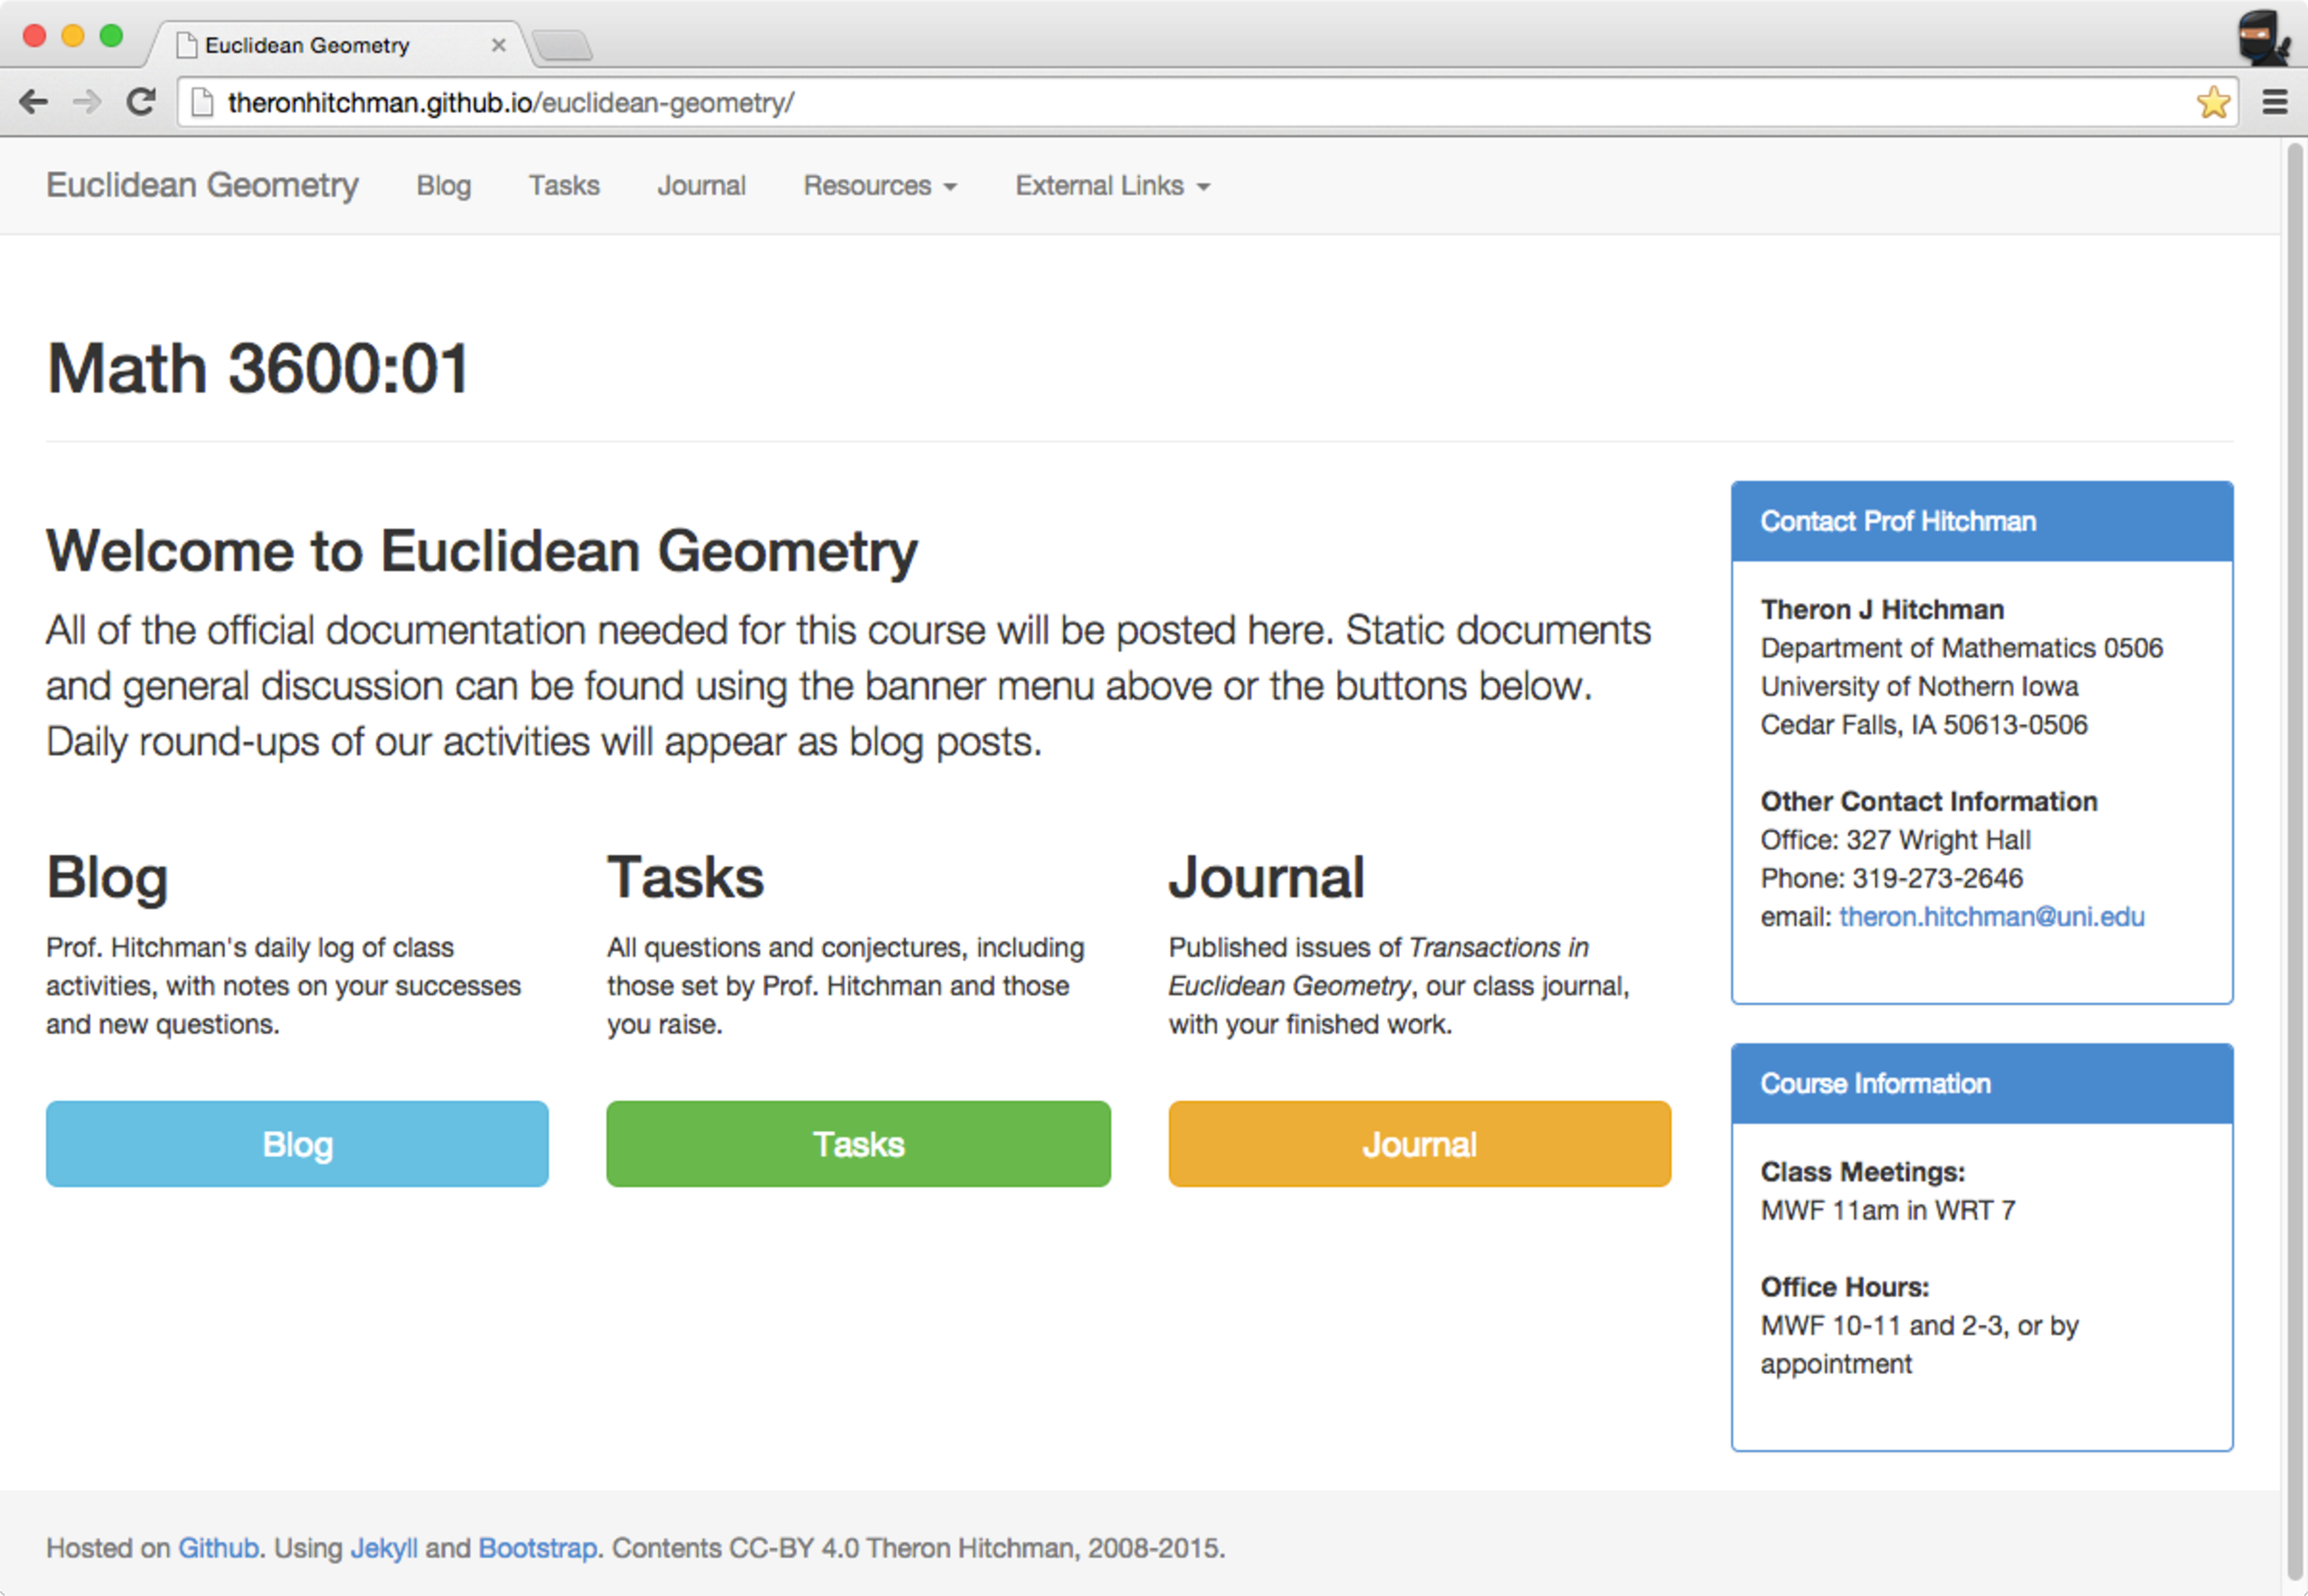
\includegraphics[width=.5\linewidth]{EGweb}
        \end{block}

        \begin{block}{\centering {\Large Linear Algebra}}
          \centering
            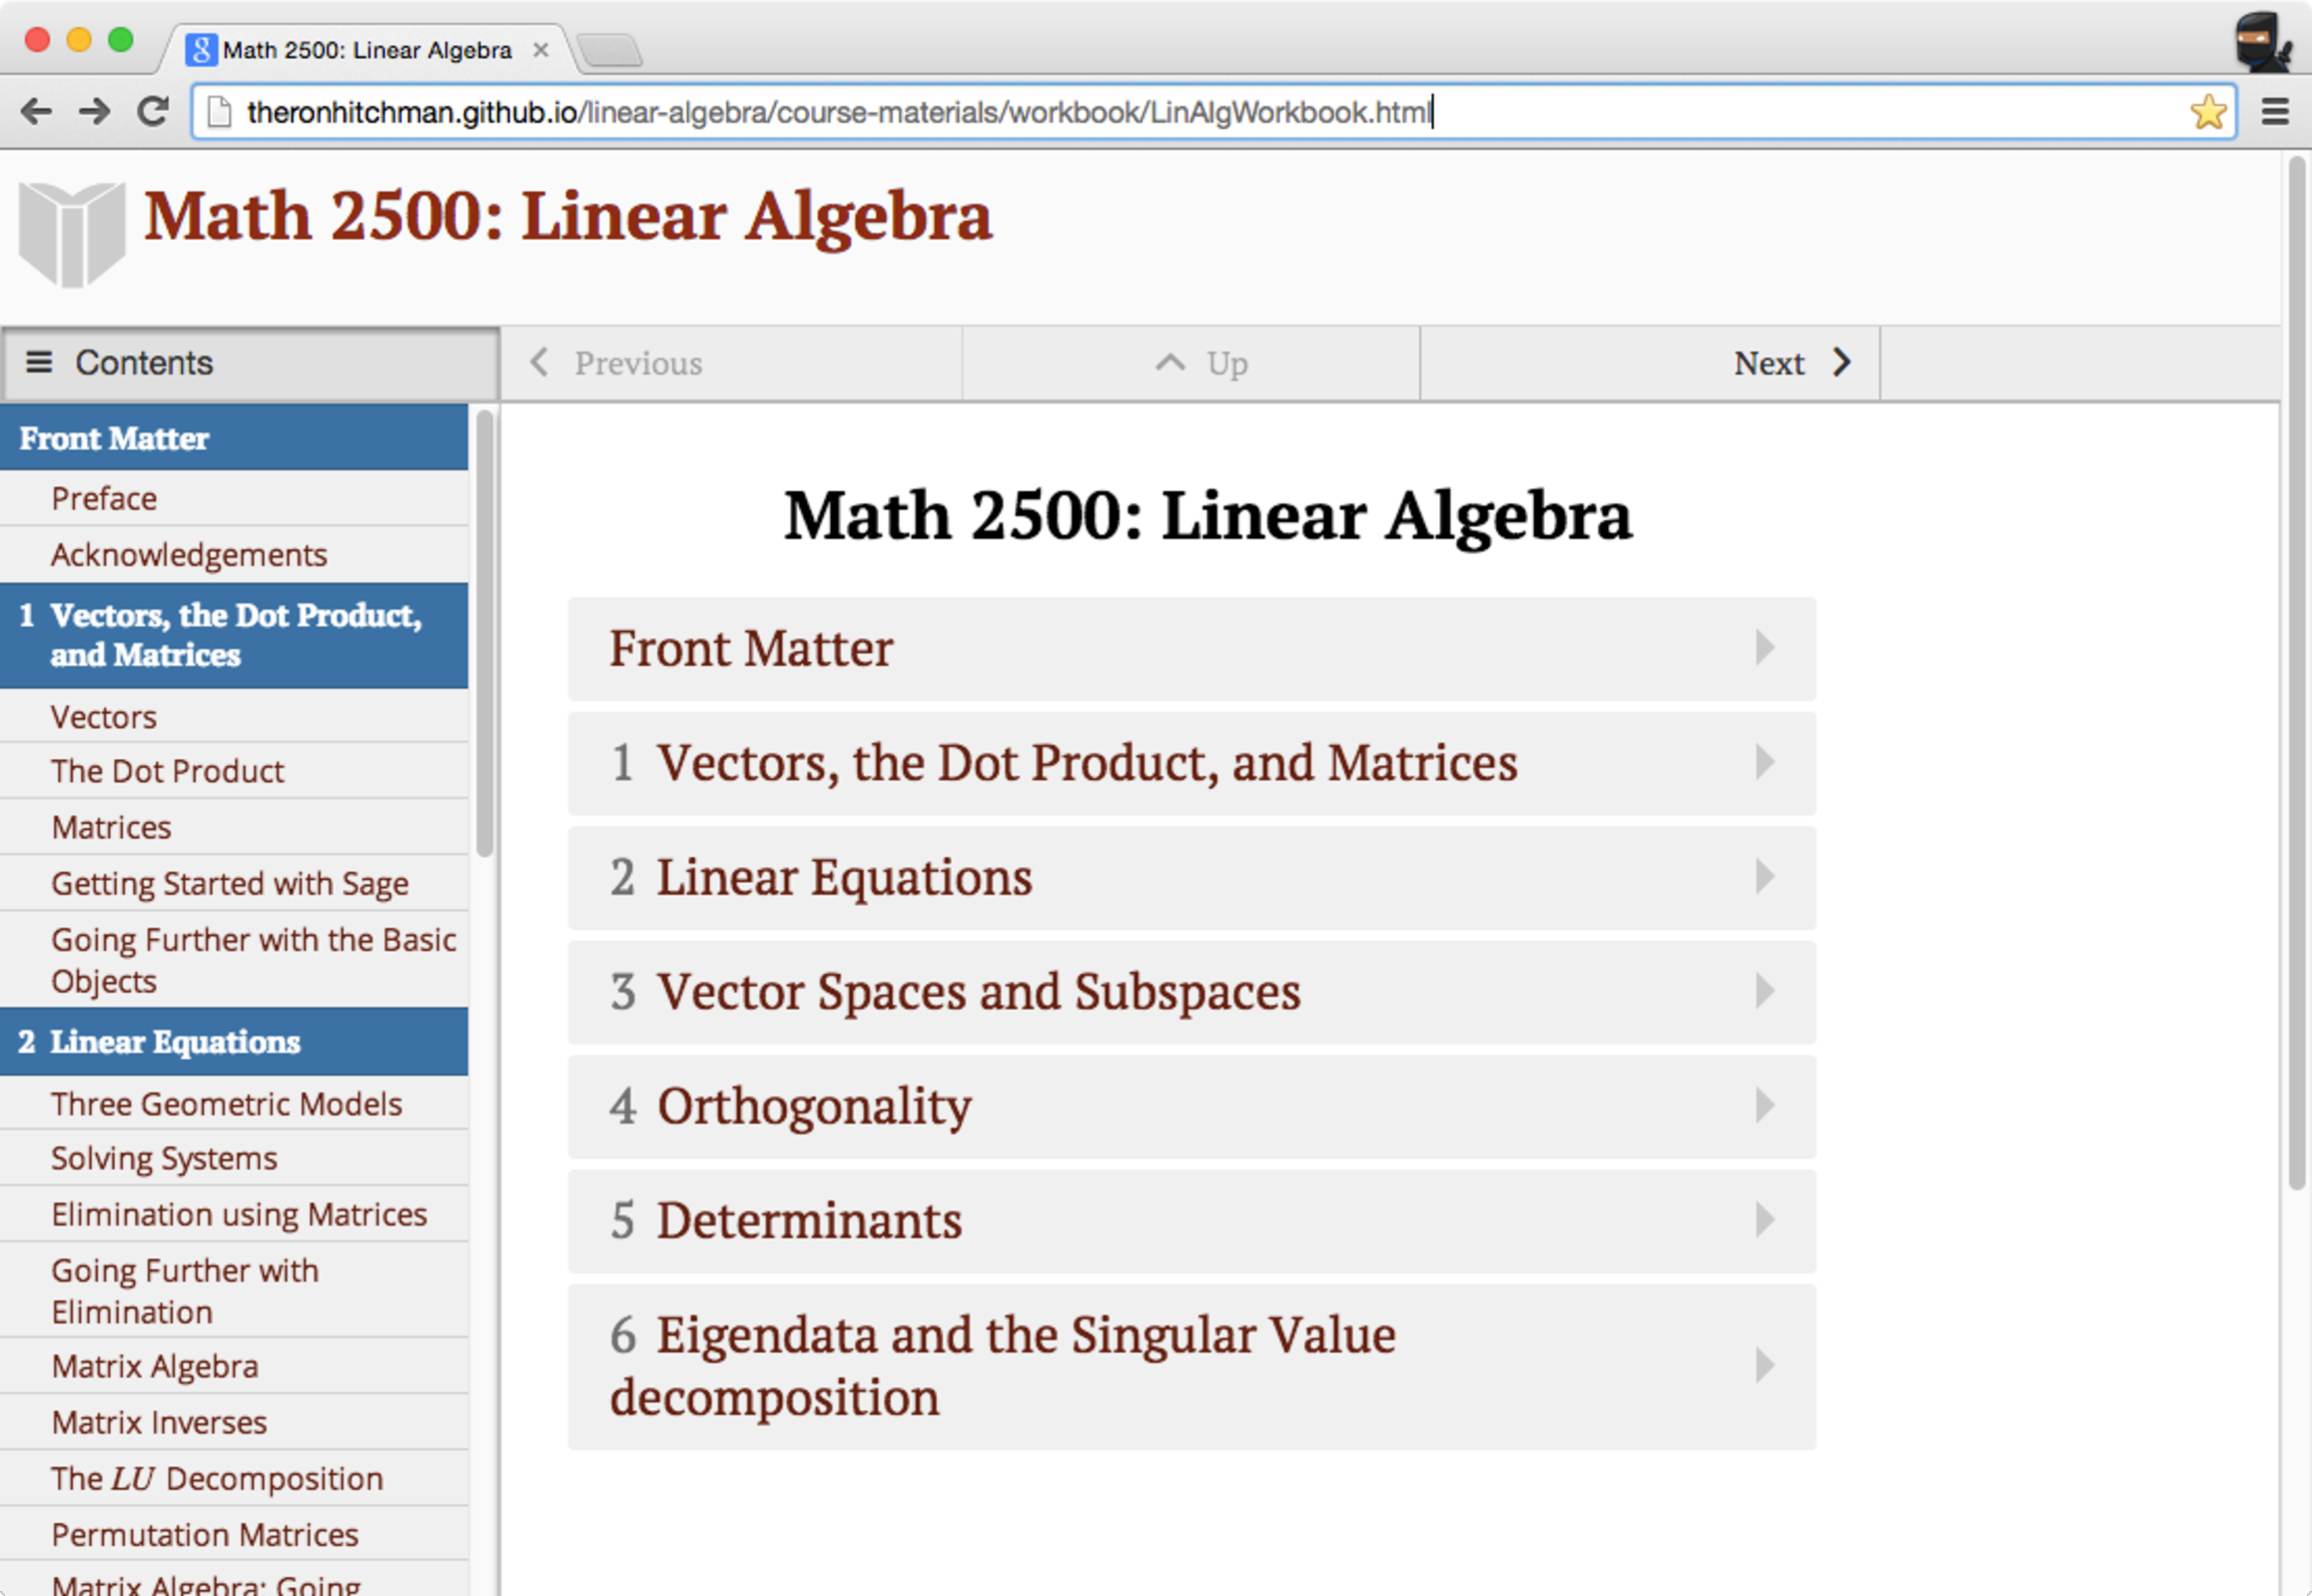
\includegraphics[width=.6\linewidth]{laworkbook}
        \end{block}
      \end{column}
    \end{columns}




  \end{frame}
  \end{document}



%%%%%%%%%%%%%%%%%%%%%%%%%%%%%%%%%%%%%%%%%%%%%%%%%%%%%%%%%%%%%%%%%%%%%%%%%%%%%%%%%%%%%%%%%%%%%%%%%%%%
%%% Local Variables: 
%%% mode: latex
%%% TeX-PDF-mode: t